\section{Estrazione e classificazione delle facce}
\label{sec:estrazione_classificazione_facce}

In questa fase l'obiettivo è rappresentare la geometria (vertici e archi) sotto forma di grafo planare embedded (PSLG) mediante la struttura Half-Edge, ed estrarre da essa le facce poligonali che costituiranno la base per la successiva triangolazione ed estrusione (Sezione \ref{sec:ricostruzione_mesh}).

Per implementare la struttura Half-Edge è stata utilizzata la libreria CGAL \cite{cgal}. Come input si passano la lista dei vertici e degli archi (\texttt{Edge}); come output si ottiene una raccolta di poligoni 2D (facce) distinti ed espliciti.

A questo punto è possibile definire la struttura di una faccia (Figura~\ref{fig:face-uml}), caratterizzata da: un vettore di vertici, i tipi di arco (layer) da cui è composta, e il tipo di faccia stesso:

\begin{figure}[H]
	\centering
	\begin{tikzpicture}
		\begin{class}[text width=7cm]{Face}{0,0}
			\attribute{- vertices : Point [*]}
			\attribute{- edgeLayers : SegmentLayer [*]}
			\attribute{- type : FaceType}
		\end{class}
		\begin{class}[text width=4cm]{FaceType}{8,0}
			\operation{<<enumeration>>}
			None=0, Floor, Window, Door, Wall
			\attribute{Unknown}
			\attribute{Floor}
			\attribute{Window}
			\attribute{Door}
			\attribute{Wall}
		\end{class}
		
	\end{tikzpicture}
	\caption{Diagramma UML della classe \texttt{Face}, che rappresenta una faccia del grafo con i relativi vertici, la semantica degli archi e il tipo di faccia.}
	\label{fig:face-uml}
\end{figure}

Si itera quindi su ogni faccia estratta, effettuandone la classificazione in base al tipo dei suoi archi. Una faccia è classificata \texttt{DOOR} se e solo se ha esattamente quattro archi: 2 \texttt{DOOR} e 2 \texttt{WALL} (Figura \ref{fig:door_polygon}). Analogamente, una faccia è classificata \texttt{WINDOW} se e solo se ha esattamente quattro archi: 2 \texttt{WINDOW} e 2 \texttt{WALL}. Una faccia è classificata \texttt{WALL} se tutti i suoi archi sono etichettati \texttt{WALL}. In tutti gli altri casi, la faccia resta non classificata.

La classificazione è fondamentale perché, come si vedrà nella Sezione \ref{sec:ricostruzione_mesh}, l'estrusione viene effettuata in modo differenziato a seconda del tipo di faccia.

Al termine di questa fase si effettua il plot delle facce estratte, per verificarne la correttezza (Figura ~\ref{fig:plot_faces}).
\begin{figure}[htbp]
	\centering
	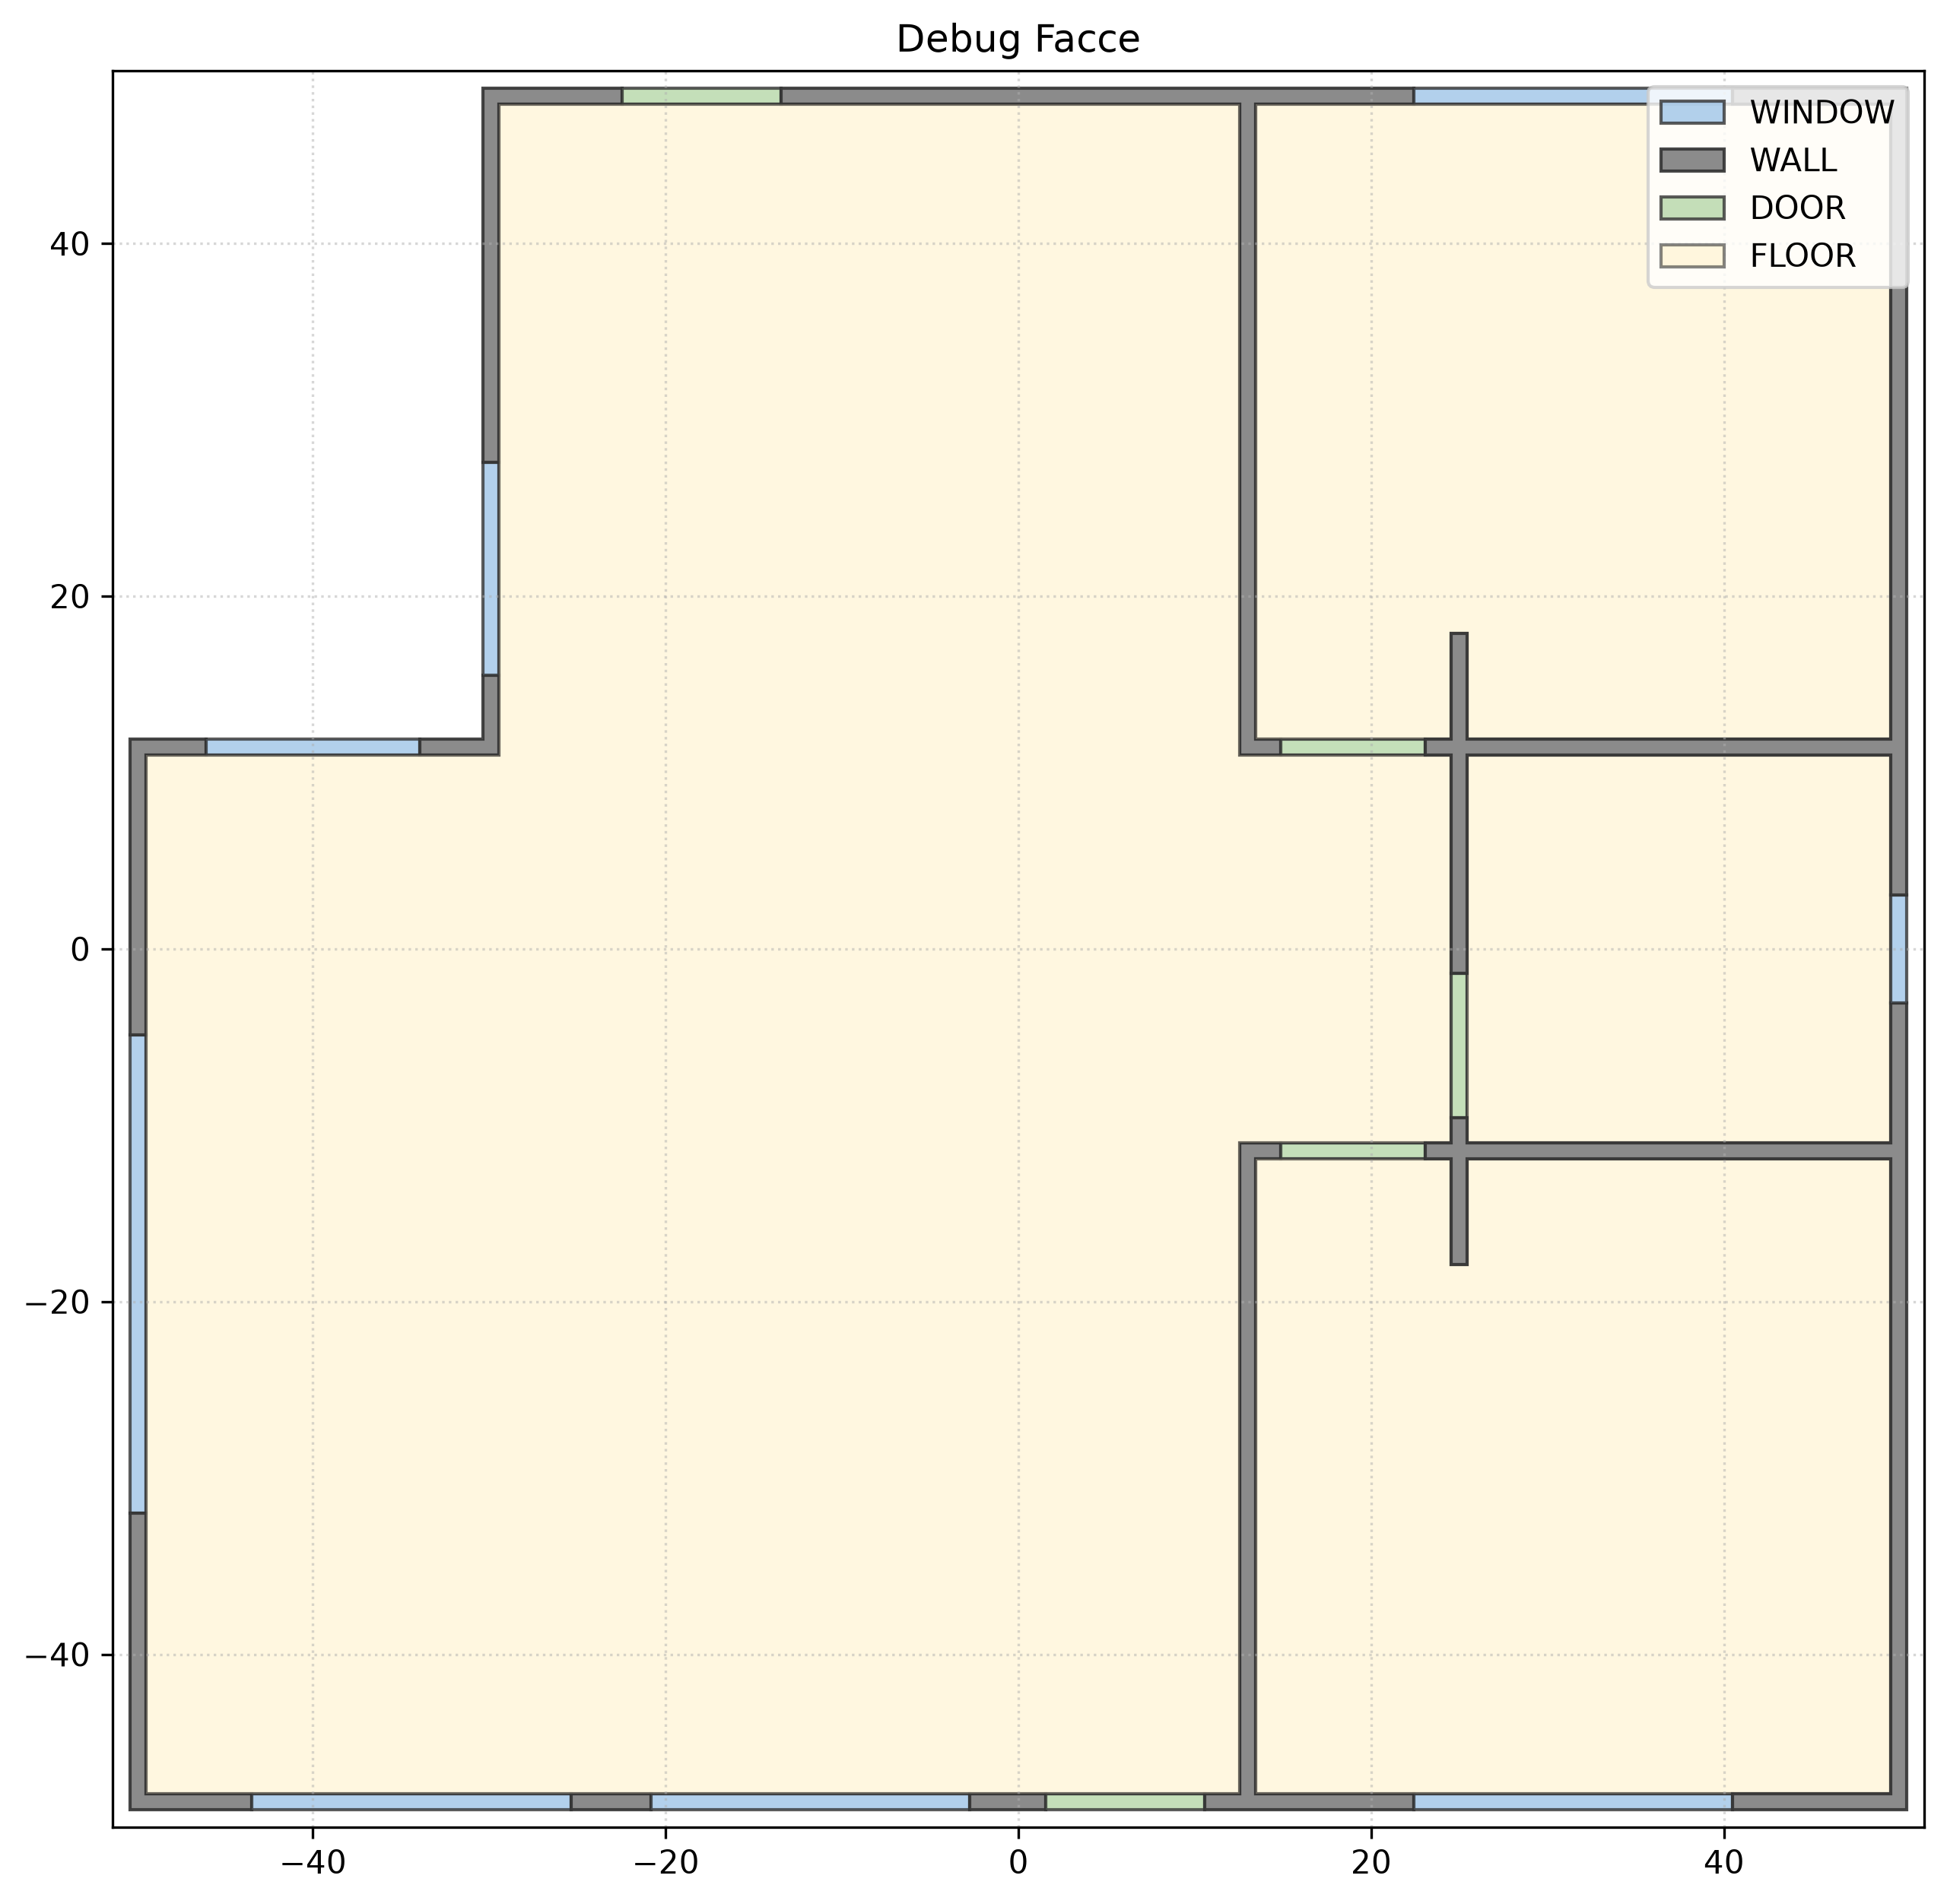
\includegraphics[width=0.75\textwidth]{figures/3_progettazione_pipeline/faces.png}
	\caption{Facce poligonali estratte dalla struttura Half-Edge a partire dal PSLG dei muri, delle porte e delle finestre.}
	\label{fig:plot_faces}
\end{figure}